\chapter{Edge Detection Experimentation}
\lhead{\emph{Edge Detection Experimentation}}

The effect of changing the size of the blur kernel was tested (Figure \ref{fig:Blur}), and it was determined that the size of the kernel has a slight effect on both the noise and edge accuracy; reducing the size makes the edges more accurate to the original at the expense of more noise, whereas increasing the size results in less noise but also less accurate edges.

\begin{figure}[H]
    \begin{center}
    \begin{tabular}{ c c c }
        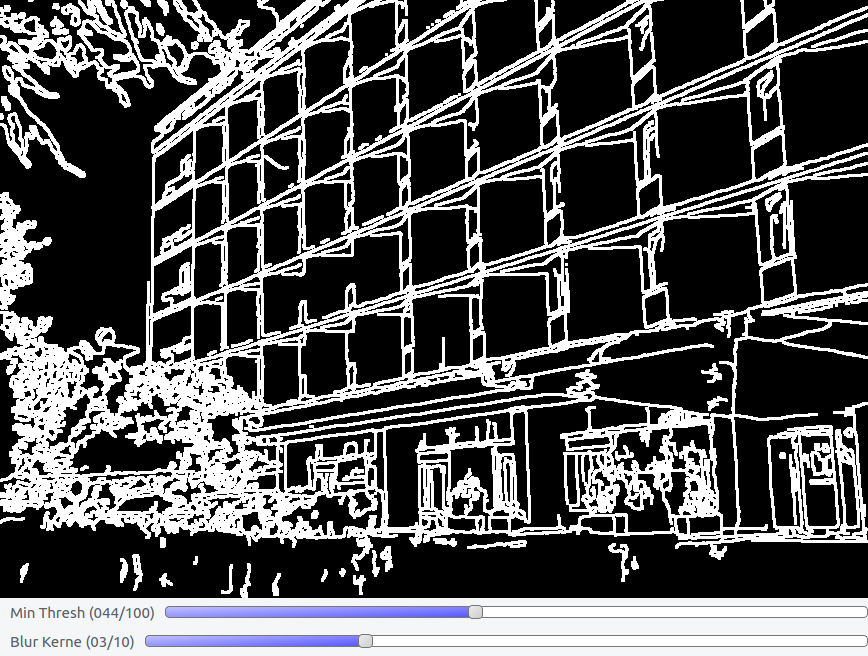
\includegraphics[width=0.31\textwidth]{Figures/Blur1.png} &
        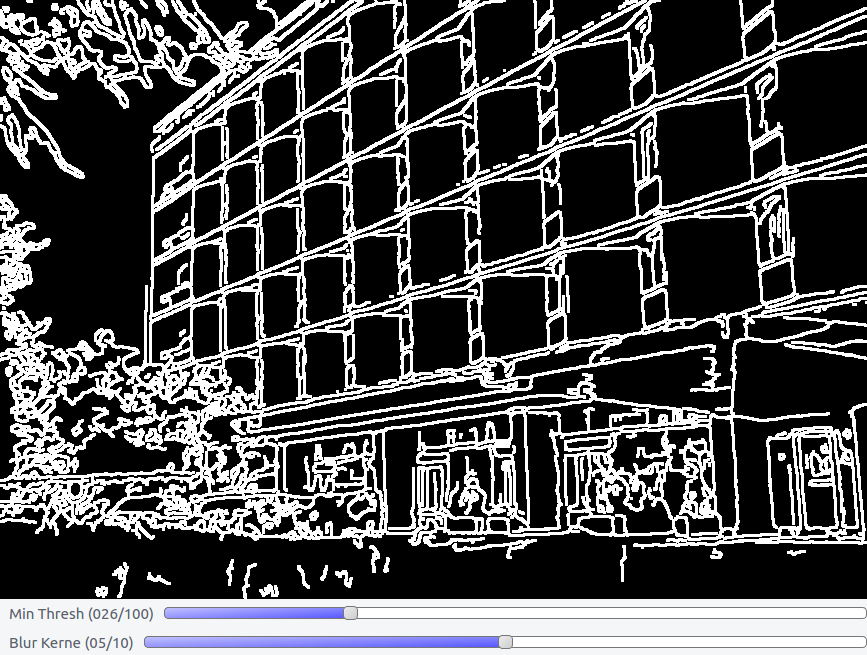
\includegraphics[width=0.31\textwidth]{Figures/Blur2.png} &
        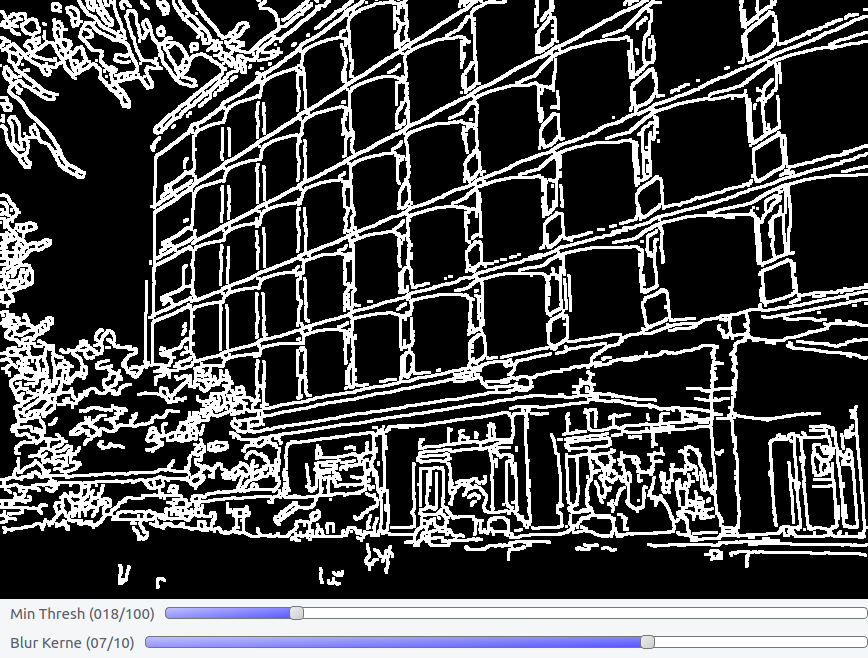
\includegraphics[width=0.31\textwidth]{Figures/Blur3.png}
    \end{tabular}
    \caption[The effect of blurring on edge detection]{The effect of blurring on edge detection. From left to right the size of the square blur kernel is increasing through 3, 5, and 7, and the lower canny threshold is decreasing through 44, 26, and 18 (the threshold change was for the purpose of presenting the best case ratio of detail to noise for each image). This figure shows the minor decrease in noise as the blur kernel increases in size, but also the minor decrease in edge accuracy; this can be seen most clearly in the bush in the bottom right of the frame for noise, and the panels on the upper right of the building for edge accuracy}
    \label{fig:Blur}
    \end{center}
\end{figure}

The edge detection function itself has 3 parameters- low threshold, high threshold, and kernel size. The kernel was set to 3x3 and the high threshold set to 3 times the low threshold by the recommendation of the OpenCV documentation \cite{cannyedgedetector}. From there the effect of changing the low threshold was tested (Figure \ref{fig:Thresh}). Increasing the threshold increased the level of detail at the expense of also increasing the noise. However, it was discerned that different situations can call for drastically different thresholds, therefore necessitating the ability to change the threshold at runtime from within the Unreal 4 environment.

\begin{figure}[H]
    \begin{center}
    \begin{tabular}{ c c }
        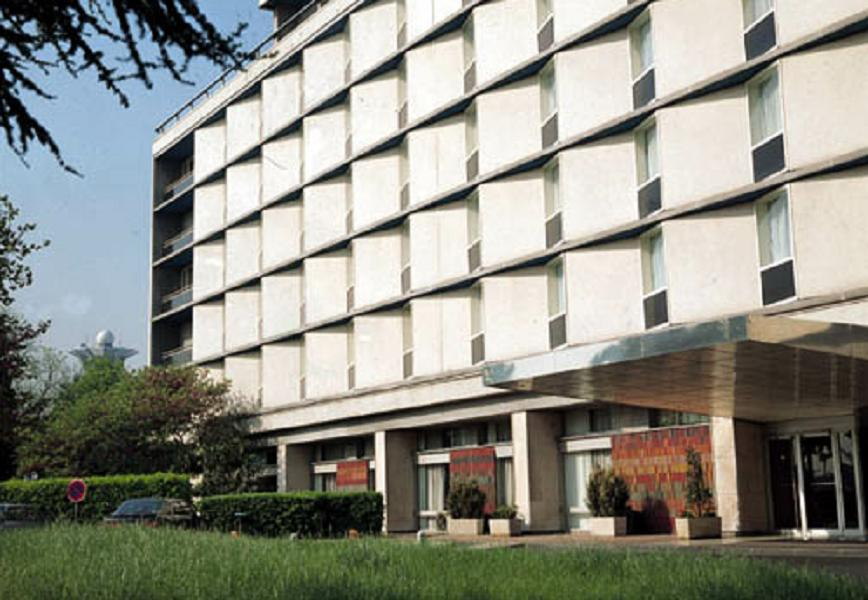
\includegraphics[width=0.405\textwidth]{Figures/building.jpg} &
        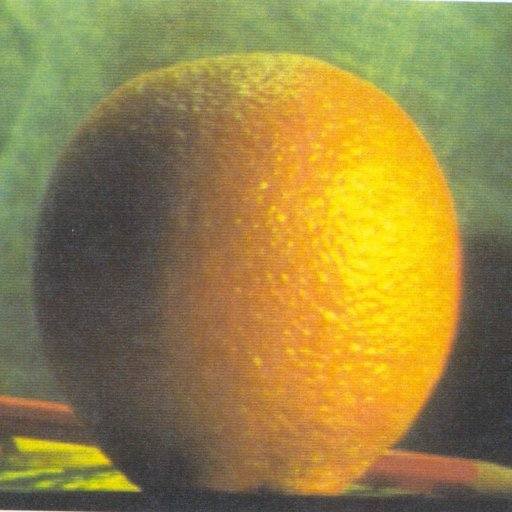
\includegraphics[width=0.28\textwidth]{Figures/orange.jpg} \\
        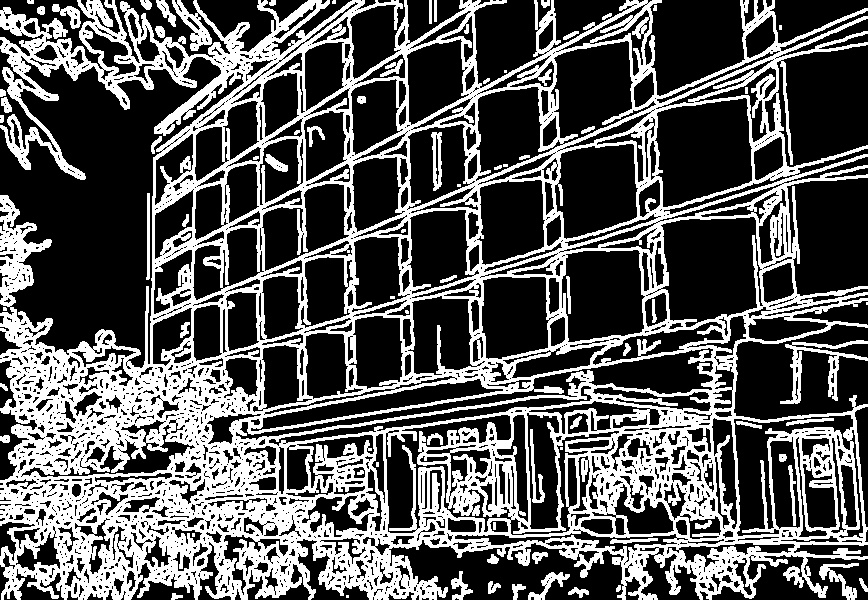
\includegraphics[width=0.405\textwidth]{Figures/buildThresh15.jpg} &
        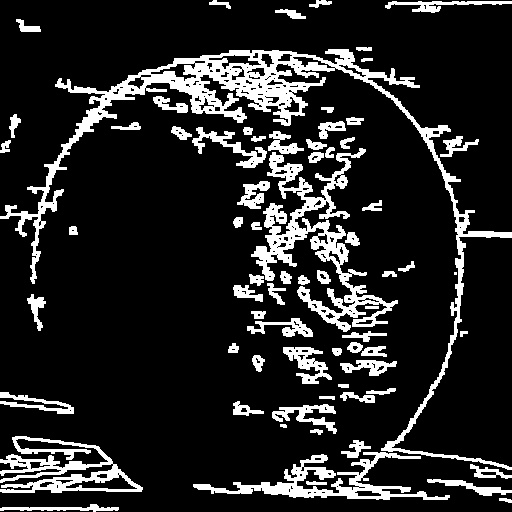
\includegraphics[width=0.28\textwidth]{Figures/orangeThresh15.jpg} \\
        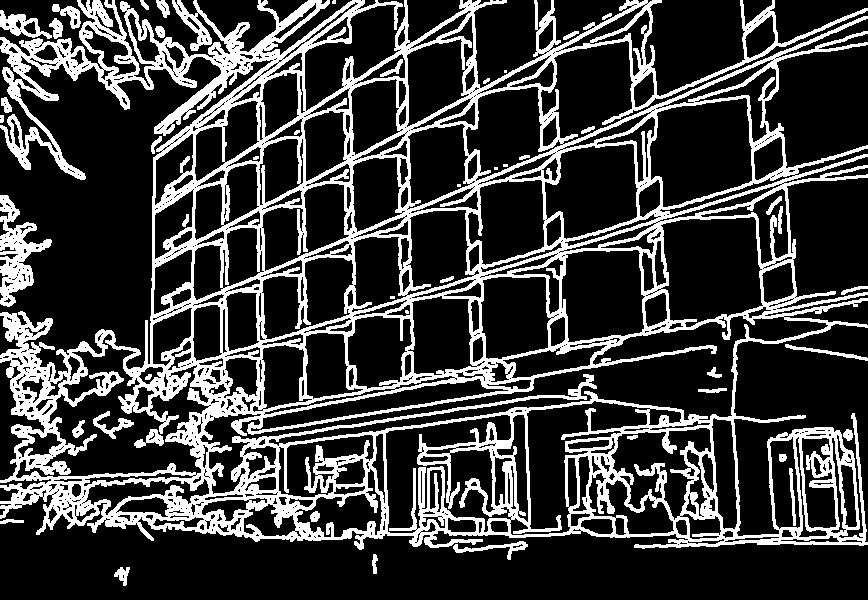
\includegraphics[width=0.405\textwidth]{Figures/buildThresh30.jpg} &
        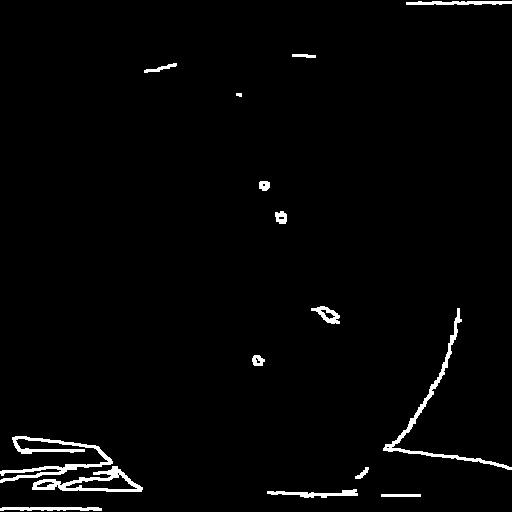
\includegraphics[width=0.28\textwidth]{Figures/orangeThresh30.jpg} \\
        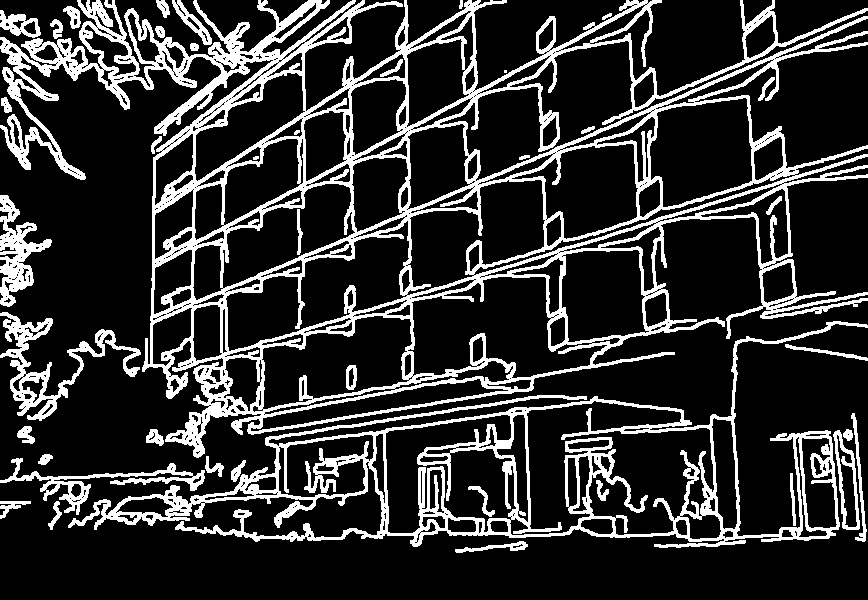
\includegraphics[width=0.405\textwidth]{Figures/buildThresh45.jpg} &
        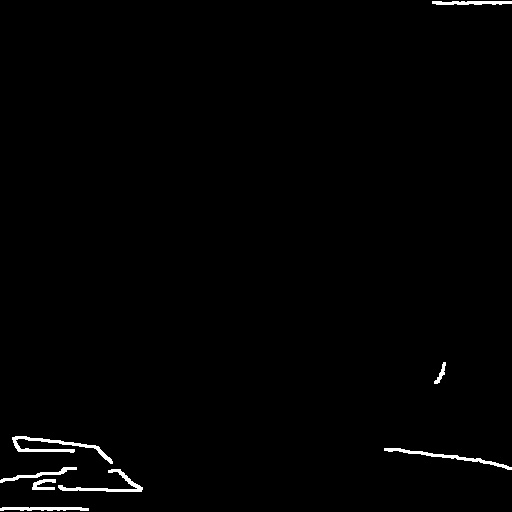
\includegraphics[width=0.28\textwidth]{Figures/orangeThresh45.jpg}
    \end{tabular}
    \caption[The effect of changing Canny threshold values]{The effect of changing Canny threshold values. From top to bottom, presented are images provided by OpenCV, then those images edge detected with low thresholds of 15, 30, and 45. The blur kernel is always 5x5 and the high threshold 3 times the low threshold. It can be seen that the best threshold for the building is 30, whereas the best for the orange is 15. This proves the necessity of being able to change the threshold at run-time to account for different situations.}
    \label{fig:Thresh}
    \end{center}
\end{figure}
